%%%%%%%%%%%%%%%%%%%%%%%%%%%%%%%%%%%%%%%%%%%%%%%%%%%%%%%%%%%%%%%%%
%
% Project     : Turnverein App
% Title       : 
% File        : anforderungsdokument.tex Rev. 00
% Date        : 07.07.14
% Author      : Raffael Santschi
%
%%%%%%%%%%%%%%%%%%%%%%%%%%%%%%%%%%%%%%%%%%%%%%%%%%%%%%%%%%%%%%%%%

\chapter{Anforderungsdokument}\label{chap.anforderungsdokument}

Das Anforderungsdokument legt den Grundstein für die Implementation. Es lohnt sich, detaillierte Anforderungen zu erfassen. Einerseits beugt dies vor möglichen Missverständnissen vor, andererseits ist es eine Absicherung, falls am Ende eines Projektes unterschiedliche Ansichten über den Lieferumfang bestünden.

\section{Übersicht}\label{anf_uebersicht}

In diesem Abschnitt werden die System- und Kontextabgrenzung dargelegt, die Systemumgebung beschrieben, die getroffenen Annahmen festgehalten und die verschiedenen \glossarmark{Stakeholder} mit ihren Erwartungen aufgelistet.

\subsection{System- und Kontextabgrenzung}\label{systemabgrenzung}
Der Systemkontext umfasst alle Aspekte, die für die Anforderungen des geplanten Systems relevant sind und nicht im Rahmen der Entwicklung dieses System gestaltet werden können.

Das geplante System hat zwei relevante Schnittstellen zur Aussenwelt, welche die Applikation beeinflussen. Die beiden Push Notification Services \glossarmark{Apple Push Notification Service} (\glossarmark{APNS}) und \glossarmark{Google Cloud Messaging for Android} (\glossarmark{GCM}). Des Weiteren wird das System von den verschiedenen Smartphone Typen, dem Anmeldeprozess, dem Hosting und, nicht zu vergessen, den Mitgliedern beeinflusst.

\cite{req_eng_book} 
\begin{figure}[h]
\centering
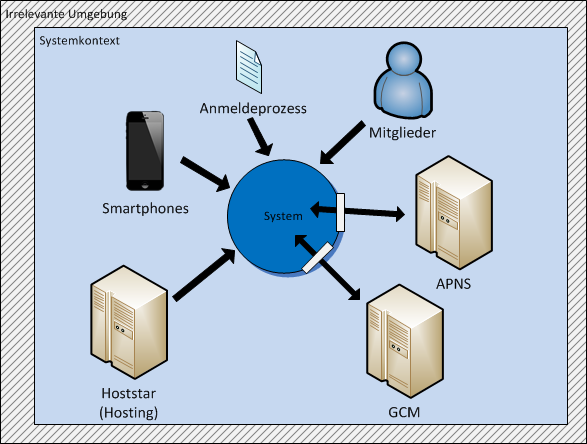
\includegraphics[scale=0.8]{images/visio/systemkontext.png}
\caption{Systemkontext}
\label{fig:systemkontext}
\end{figure}

\FloatBarrier
\subsection{Systemumgebung}\label{systemumgebung}
Die Systemumgebung definiert die Ausgangslage für ein Projekt. Am Anfang des Projekts bestand das System aus einem Webserver, auf dem ein \glossarmark{PHP} Backend und eine interaktive Webseite liefen. Die Daten wurden in einer MySQL Datenbank abgespeichert. 

Die Seite wird rege benutzt, es sind etwa 35 Benutzer pro Tag online. Fast jedes Mitglied besitzt ein Smartphone, wobei die Aufteilung zwischen Android und iOS Geräten etwa ausgeglichen ist. In Abbildung \ref{fig:systemumgebung} ist die Systemumgebung graphisch dargestellt.
\begin{figure}[h]
\centering
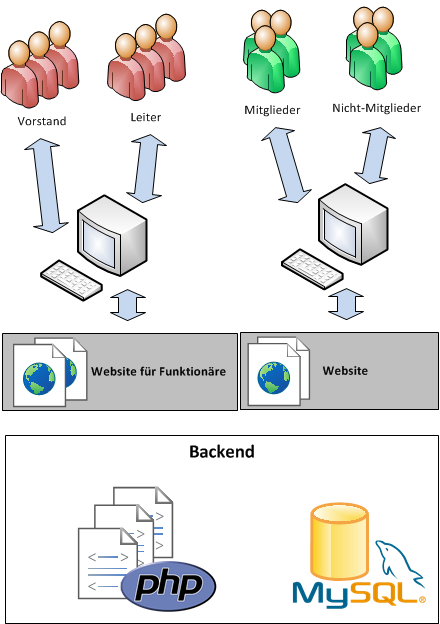
\includegraphics[scale=0.95]{images/visio/systemumgebung.png}
\caption{Systemumgebung}
\label{fig:systemumgebung}
\end{figure}

\FloatBarrier
\subsection{Annahmen}\label{annahmen}
Es mussten keine Annahmen getroffen werden, da durch die enge Zusammenarbeit mit dem Turnverein, alle offenen Punkte in kürzester Zeit geklärt werden konnten.

\newpage
\subsection{Stakeholder}\label{stakeholder}
Die \glossarmark{Stakeholder} Analyse dient dem erfassen aller Nutzergruppen, die auf ein Projekt Einfluss haben. Zudem ermöglicht sie die Erfassung aller Gruppen, die potentiell Anforderungen an das Projekt stellen. In der der Tabelle \ref{table:stakeholder} wurden die \glossarmark{Stakeholder} für dieses Projekt mit der Hilfe des Vorstandes zusammengetragen und ihre Erwartungen, ihre Einstellung und ihr Einfluss gegenüber diesem Projekt festgehalten\footnote{Obwohl in diesem Projekt primär die Bedürfnisse des Turnvereins betrachtet werden, soll die App auch für den Damenturnverein und die Jugensport Kommission nutzbar sein.}. 

\begin{table}[ht]
\centering
  \begin{tabular}{ l | p{5cm} | p{1.5cm} | p{1.5cm} }
	\hline
	\rowcolor{darkgray}
	\textbf{Name}					&	\textbf{Erwartung}	&	\textbf{Einstellung} 	&	\textbf{Einfluss}	\\ \hline
	\rowcolor{gray}
								&				&	-Positiv \mbox{-Neutral} \mbox{-Negativ} 	&	-Hoch \mbox{-Mittel} \mbox{-Niedrig} \\ \hline
	Vorstand						&	Der Vorstand ist der Kunde in diesem Projekt, er hat den Auftrag erteilt. Er erwartet von der App mehr Popularität, vor allem bei den jüngeren Mitgliedern. Zusätzlich erhofft er sich etwas Werbung für den Verein.			
												& 	Positiv		&	Hoch		\\ \hline
	Trainingsverantwortliche				&	Die Trainingsverantwortlichen sehen einen grossen Vorteil darin, dass die Anmeldung für die Trainings vereinfacht werden soll. Sie finden es praktisch, dass sie die Trainingsinformationen schnell abrufen können.			
												& 	Positiv		&	Hoch		\\ \hline
	aktive Mitglieder (U30)				&	Die jüngere Generation der aktiv Mitglieder wartet gespannt auf die App.	Sie wünschen sich eine schnelle Möglichkeit sich anmelden zu können.		
												& 	Positiv		&	Hoch		\\ \hline
	aktive Mitglieder (Ü30)				&	Die ältere Generation der aktiv Mitglieder hat keine grossen Erwartungen an die App, sie würden auch ohne auskommen.		
												& 	Neutral	&	Mittel		\\ \hline
	Passiv- und Ehrenmitglieder			&	Passiv- und Ehrenmitglieder gehören auch eher zu dem älteren Semester und können mit Apps nicht viel anfangen. Sie sind der App gegenüber jedoch nicht negativ eingestellt. Da diese Gruppe einen hohen Einfluss besitzt, ist dies sehr von Vorteil.
												& 	Neutral	&	Hoch		\\ \hline
	Nicht-Mitglieder					&	Die Nicht-Mitglieder erhoffen sich schnelle und gute Informationen über Anlässe und die Vereine selbst.
												& 	Neutral	&	Niedrig	\\ \hline
  \end{tabular}
   \caption{Liste der evaluierten Stakeholder}\label{table:stakeholder}
\end{table}

\newpage
\section{Anforderungen}\label{sec.anfoderungen}
Beim Erfassen der Anforderungen wurden als Erstes die Use-Cases definiert. Diese wurden zusammen mit Vertretern des Turnvereins festgelegt. Die Beschreibung beinhaltet bereits einen klaren Ablauf für die einzelnen Use-Cases. Als nächstes wurden in mehreren Sitzungen die dazugehörigen \glossarmark{Mockups} gestaltet. Bevor die Implementation beginnen konnte, mussten noch die Anforderungen abgeleitet werden. Sie wurden auf der Grundlage einer Mitglieder Befragung und einer kurzen Sitzung mit dem Vorstand evaluiert.

\subsection{Use Cases}\label{use_cases}
Das Use Case Diagramm (siehe Abbildung \ref{fig:use_case}) zeigt zwei Akteure, Mitglieder und Nicht-Mitglieder, sowie sechs Use Cases, welche in diesem Projekt umgesetzt wurden.
\begin{figure}[h]
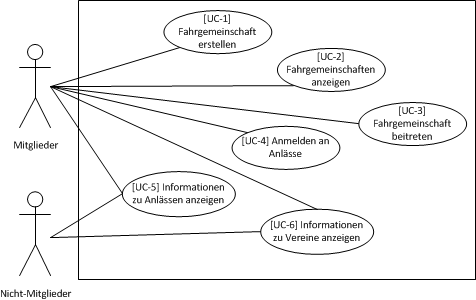
\includegraphics{images/anforderungen/use_cases.png}
\caption{Use-Case Diagramm}
\label{fig:use_case}
\end{figure}

Alle Use Cases wurden anhand der folgenden Vorlage in Tabelle \ref{table:use_case_template} spezifiziert. Diese Schablone basiert auf Angaben von \cite{req_eng_book}. Die Use Cases wurden möglichst genau beschrieben, was danach die Implementation vereinfachte.

\begin{table}[ht]
\centering
  \begin{tabular}{ l | p{10cm} }
	\hline
	\rowcolor{gray}
	\textbf{Bezeichner}		&	Eindeutiger Bezeichner\\ \hline
	\textbf{Name}			&	Eindeutiger Name\\ \hline
	\textbf{Kritikalität}		&	Kritikalität hinsichtlich des Schadensausmasses bei Fehlverhalten: hoch, mittel, leicht\\ \hline
	\textbf{Quelle}			&	\glossarmark{Stakeholder}, Dokument, System\\ \hline
	\textbf{Verantwortlicher}	&	Verantwortlicher \glossarmark{Stakeholder}\\ \hline
	\textbf{Beschreibung}	&	Komprimierte Beschreibung\\ \hline
	\textbf{Auslösendes Ereignis}&	Angabe des Ereignisses, das den Use Case auslöst\\ \hline
	\textbf{Akteure}		&	Auflistung der Akteure, die mit dem Use Case in Beziehung stehen\\ \hline
	\textbf{Vorbedingung}	&	Eine Liste notwendiger Voraussetzungen, die erfüllt sein müssen, bevor die Ausführung des Use Case beginnen kann\\ \hline
	\textbf{Nachbedingung}	&	Eine Liste von Zuständen, in denen sich das System unmittelbar nach der Ausführung des Hauptszenarios befindet.\\ \hline
	\textbf{Ergebnis}		&	Beschreibung der Ausgaben, die während der Ausführung des Use Case erzeugt werden\\ \hline
	\textbf{Hauptszenario}	&	Beschreibung des Hauptszenarios eines Use Case\\ \hline
	\textbf{Alternativszenarien}	&	Beschreibung von Alternativszenarien des Use Case oder lediglich Angabe der auslösenden Ereignisse. 
					Hier gelten oftmals andere Nachbedingungen.\\ \hline
	\textbf{Ausnahmeszenarien}&	Beschreibung von Ausnahmeszenarien des Use Case oder lediglich Angabe der auslösenden Ereignisse. 
					Hier gelten oftmals andere Nachbedingungen.\\ \hline
	\textbf{Mockups}	 	&	Querbezüge zu \glossarmark{Mockups}
  \end{tabular}
   \caption{Vorlage für Use Case Spezifikation}\label{table:use_case_template}
\end{table}

\begin{table}[ht]
\centering
  \begin{tabular}{ l | p{10cm} }
	\hline
	\rowcolor{gray}
	\textbf{Bezeichner}		&	\textbf{UC-1}\\ \hline
	\textbf{Name}			&	Fahrgemeinschaft erstellen\\ \hline
	\textbf{Kritikalität}		&	hoch\\ \hline
	\textbf{Quelle}			&	\glossarmark{Stakeholder}\\ \hline
	\textbf{Verantwortlicher}	&	Marco Mathe (Vorstand)\\ \hline
	\textbf{Beschreibung}	&	Eine der Hauptaufgaben dieser App soll die Fahrgemeinschaftsverwaltung sein. Jedes Mitglied soll eine Fahrgemeinschaft erstellen können.\\ \hline
	\textbf{Auslösendes Ereignis}&	Mitglied möchte eine Fahrgemeinschaft erstellen\\ \hline
	\textbf{Akteure}		&	TV-Mitglied\\ \hline
	\textbf{Vorbedingung}	&	Das Mitglied ist angemeldet und es existiert eine Veranstaltung\\ \hline
	\textbf{Nachbedingung}	&	Das Mitglied hat eine Fahrgemeinschaft erstellt\\ \hline
	\textbf{Ergebnis}		&	Erstellung einer neuen Fahrgemeinschaft\\ \hline
	\textbf{Hauptszenario}	&	\begin{enumerate}
					\item Das Mitglied öffnet den Menü-Knopf
					\item Das System zeigt das Menü an
					\item Das Mitglied klickt auf eine der drei Veranstaltungstypen
					\item Das System fragt eine Liste der Veranstaltungen beim Backend ab
					\item Das System zeigt eine Liste der Veranstaltungen an
					\item Das Mitglied sucht die Veranstaltung und klickt darauf
					\item Das Mitglied klickt auf 'Fahrgemeinschaften'
					\item Das Mitglied klickt auf 'Neue Fahrgemeinschaft'
					\item Das System zeigt ein Formular mit Daten zur Fahrgemeinschaft an
					\item Das Mitglied füllt die Felder aus und sendet das Formular ab
					\item Das System schickt die Daten an das Backend
					\item Das System zeigt 'Fahrgemeinschaft erfolgreich erstellt' an
					\end{enumerate}
					\\ \hline
	\textbf{Alternativszenarien}	&	\begin{enumerate}
					\item[7a] Das System weist das Mitglied auf fehlende Felder hin
					\end{enumerate}
					\\ \hline
	\textbf{Ausnahmeszenarien}&	\begin{enumerate}
					\item[7a] Das System zeigt 'keine Internetverbindung vorhanden' an
					\end{enumerate}
					\\ \hline
	\textbf{Mockups}	 	&	-
  \end{tabular}
   \caption{Use Case UC-1: Fahrgemeinschaft erstellen}\label{table:use_case_1}
\end{table}

\begin{table}[ht]
\centering
  \begin{tabular}{ l | p{10cm} }
	\hline
	\rowcolor{gray}
	\textbf{Bezeichner}		&	\textbf{UC-2}\\ \hline
	\textbf{Name}			&	Fahrgemeinschaften anzeigen\\ \hline
	\textbf{Kritikalität}		&	hoch\\ \hline
	\textbf{Quelle}			&	\glossarmark{Stakeholder}\\ \hline
	\textbf{Verantwortlicher}	&	Marco Mathe (Vorstand)\\ \hline
	\textbf{Beschreibung}	&	Eine der Hauptaufgaben dieser App soll die Fahrgemeinschaftsverwaltung sein. Die Mitglieder sollen sich eine Liste aller Fahrgemeinschaften anzeigen lassen können, um dann zu entscheiden, welcher sie sich anschliessen möchten.\\ \hline
	\textbf{Auslösendes Ereignis}&	Mitglied möchte Fahrgemeinschaften anschauen\\ \hline
	\textbf{Akteure}		&	TV-Mitglied\\ \hline
	\textbf{Vorbedingung}	&	Das Mitglied ist angemeldet und Fahrgemeinschaften sind vorhanden\\ \hline
	\textbf{Nachbedingung}	&	Das Mitglied hat eine Liste von Fahrgemeinschaften erhalten\\ \hline
	\textbf{Ergebnis}		&	Liste von Fahrgemeinschaften\\ \hline
	\textbf{Hauptszenario}	&	\begin{enumerate}
					\item Das Mitglied öffnet den Menü-Knopf
					\item Das System zeigt das Menü an
					\item Das Mitglied klickt auf eine der drei Veranstaltungstypen
					\item Das System fragt eine Liste der Veranstaltungen beim Backend ab
					\item Das System zeigt eine Liste der Veranstaltungen an
					\item Das Mitglied sucht die Veranstaltung und klickt darauf
					\item Das Mitglied klickt auf 'Fahrgemeinschaften'
					\item Das System fragt eine Liste der Fahrgemeinschaften beim Backend ab
					\item Das System zeigt eine Liste der Fahrgemeinschaften an
					\end{enumerate}
					\\ \hline
	\textbf{Alternativszenarien}	&	\begin{enumerate}
					\item[5a] Das System zeigt 'keine aktuellen Fahrgemeinschaften' an
					\end{enumerate}
					\\ \hline
	\textbf{Ausnahmeszenarien}&	\begin{enumerate}
					\item[4a] Das System zeigt 'keine Internetverbindung vorhanden' an
					\end{enumerate}
					\\ \hline
	\textbf{Mockups}	 	&	\ref{fig:mockup_navigation}, \ref{fig:mockup_carpools}, \ref{fig:mockup_carpool_detail},
					\ref{fig:mockup_add_carpool}
  \end{tabular}
   \caption{Use Case UC-2: Fahrgemeinschaften anzeigen}\label{table:use_case_2}
\end{table}


\begin{table}[ht]
\centering
  \begin{tabular}{ l | p{10cm} }
	\hline
	\rowcolor{gray}
	\textbf{Bezeichner}		&	\textbf{UC-3}\\ \hline
	\textbf{Name}			&	Fahrgemeinschaft beitreten\\ \hline
	\textbf{Kritikalität}		&	hoch\\ \hline
	\textbf{Quelle}			&	\glossarmark{Stakeholder}\\ \hline
	\textbf{Verantwortlicher}	&	Marco Mathe (Vorstand)\\ \hline
	\textbf{Beschreibung}	&	Eine der Hauptaufgaben dieser App soll die Fahrgemeinschaftsverwaltung sein. Beim Beitreten einer Fahrgemeinschaft geht es darum, dass das Mitglied Interesse an der Fahrgemeinschaft hat und dieser gern beitreten möchte.\\ \hline
	\textbf{Auslösendes Ereignis}&	Mitglied möchte einer Fahrgemeinschaft beitreten\\ \hline
	\textbf{Akteure}		&	TV-Mitglied\\ \hline
	\textbf{Vorbedingung}	&	Das Mitglied ist angemeldet und Fahrgemeinschaften sind vorhanden\\ \hline
	\textbf{Nachbedingung}	&	Das Mitglied ist einer Fahrgemeinschaft beigetreten\\ \hline
	\textbf{Ergebnis}		&	Neuer Eintrag in der Gemeinschaft und Kapazitätenminderung\\ \hline
	\textbf{Hauptszenario}	&	\begin{enumerate}
					\item Das Mitglied öffnet den Menü-Knopf
					\item Das System zeigt das Menü an
					\item Das Mitglied klickt auf eine der drei Veranstaltungstypen
					\item Das System fragt eine Liste der Veranstaltungen beim Backend ab
					\item Das System zeigt eine Liste der Veranstaltungen an
					\item Das Mitglied sucht die Veranstaltung und klickt darauf
					\item Das Mitglied klickt auf 'Fahrgemeinschaften'
					\item Das System zeigt eine Liste aller Fahrgemeinschaften an
					\item Das Mitglied wählt eine aus und klickt auf 'Beitreten'
					\item Das System zeigt 'Erfolgreich beigetreten' an
					\end{enumerate}
					\\ \hline
	\textbf{Alternativszenarien}	&	\begin{enumerate}
					\item[3a] Das System zeigt 'Kein Platz mehr' an
					\item[4] Der User wählt eine andere Fahrgemeinschaft aus und versucht es erneut
					\end{enumerate}
					\\ \hline
	\textbf{Ausnahmeszenarien}&	\begin{enumerate}
					\item[3a] Das System zeigt 'keine Internetverbindung vorhanden' an
					\end{enumerate}
					\\ \hline
	\textbf{Mockups}	 	&	\ref{fig:mockup_navigation}, \ref{fig:mockup_carpools}, \ref{fig:mockup_carpool_detail}
  \end{tabular}
   \caption{Use Case UC-3: Fahrgemeinschaft beitreten}\label{table:use_case_3}
\end{table}

\begin{table}[ht]
\centering
  \begin{tabular}{ l | p{10cm} }
	\hline
	\rowcolor{gray}
	\textbf{Bezeichner}		&	\textbf{UC-4}\\ \hline
	\textbf{Name}			&	Anmelden an Anlässe\\ \hline
	\textbf{Kritikalität}		&	hoch\\ \hline
	\textbf{Quelle}			&	\glossarmark{Stakeholder}\\ \hline
	\textbf{Verantwortlicher}	&	Dominic Keller (aktive Mitglieder (U30))\\ \hline
	\textbf{Beschreibung}	&	Die bekannte Anmelde-Funktion von der Homepage soll es auch in der App geben.\\ \hline
	\textbf{Auslösendes Ereignis}&	Mitglied möchte sich für einen Anlass anmelden\\ \hline
	\textbf{Akteure}		&	TV-Mitglied\\ \hline
	\textbf{Vorbedingung}	&	Das Mitglied ist angemeldet\\ \hline
	\textbf{Nachbedingung}	&	Das Mitglied hat sich für einen Anlass angemeldet\\ \hline
	\textbf{Ergebnis}		&	Erstellung einer neuen Anmeldung für den Anlass\\ \hline
	\textbf{Hauptszenario}	&	\begin{enumerate}
					\item Das Mitglied öffnet den Menü-Knopf
					\item Das System zeigt das Menü an
					\item Das Mitglied klickt auf 'Anlässe'
					\item Das System fragt eine Liste der Anlässe beim Backend ab
					\item Das System zeigt eine Liste der Anlässe an
					\item Das Mitglied sucht den Anlass und klickt darauf
					\item Das Mitglied klickt auf 'Anmelden'
					\item Das System schickt die Anmeldung zum Backend
					\item Das System zeigt 'Anmeldung erfolgreich' an
					\end{enumerate}
					\\ \hline
	\textbf{Alternativszenarien}	&	\begin{enumerate}
					\item[7a] Das Mitglied sucht den Anlass und kann nicht auf 'Anmelden' klicken, da es bereits angemeldet ist
					\end{enumerate}
					\\ \hline
	\textbf{Ausnahmeszenarien}&	\begin{enumerate}
					\item[8a] Das System zeigt 'keine Internetverbindung vorhanden' an
					\end{enumerate}
					\\ \hline
	\textbf{Mockups}	 	&	\ref{fig:mockup_navigation}, \ref{fig:mockup_events}, \ref{fig:mockup_event_detail},
					\ref{fig:mockup_matches}, \ref{fig:mockup_match_detail}, \ref{fig:mockup_trainings}, 
					\ref{fig:mockup_training_detail}
  \end{tabular}
   \caption{Use Case UC-4: Anmelden an Anlässe}\label{table:use_case_4}
\end{table}

\begin{table}[ht]
\centering
  \begin{tabular}{ l | p{10cm} }
	\hline
	\rowcolor{gray}
	\textbf{Bezeichner}		&	\textbf{UC-5}\\ \hline
	\textbf{Name}			&	Informationen zu Anlässen anzeigen\\ \hline
	\textbf{Kritikalität}		&	hoch\\ \hline
	\textbf{Quelle}			&	\glossarmark{Stakeholder}\\ \hline
	\textbf{Verantwortlicher}	&	Ivan Sebastiano (Trainingsverantwortliche)\\ \hline
	\textbf{Beschreibung}	&	Neben Funktionen für die Mitglieder soll die App auch Informationen über bevorstehende Anlässe für Mitglieder und Nicht-Mitglieder zur Verfügung stellen.\\ \hline
	\textbf{Auslösendes Ereignis}&	Mitglied möchte Informationen über einen bevorstehenden Anlass abrufen\\ \hline
	\textbf{Akteure}		&	TV-Mitglied, Nicht Mitglieder\\ \hline
	\textbf{Vorbedingung}	&	Anlässe sind vorhanden\\ \hline
	\textbf{Nachbedingung}	&	Das Mitglied hat die gewünschten Informationen erhalten\\ \hline
	\textbf{Ergebnis}		&	Informationen über den bevorstehenden Anlass\\ \hline
	\textbf{Hauptszenario}	&	\begin{enumerate}
					\item Das Mitglied öffnet den Menü-Knopf
					\item Das System zeigt das Menü an
					\item Das Mitglied klickt auf 'Anlässe'
					\item Das System fragt eine Liste der Anlässe beim Backend ab
					\item Das System zeigt eine Liste der Anlässe an
					\item Das Mitglied sucht den Anlass und klickt auf ihn
					\item Das System schickt die Anfrage an das Backend
					\item Das System zeigt detaillierte Informationen über den Anlass an
					\end{enumerate}
					\\ \hline
	\textbf{Alternativszenarien}	&	\begin{enumerate}
					\item[8a] Das System zeigt detaillierte Informationen über den Anlass und spezielle Informationen für Mitglieder an
					\end{enumerate}
					\\ \hline
	\textbf{Ausnahmeszenarien}&	\begin{enumerate}
					\item[7a] Das System zeigt 'keine Internetverbindung vorhanden' an
					\end{enumerate}
					\\ \hline
	\textbf{Mockups}	 	&	\ref{fig:mockup_navigation}, \ref{fig:mockup_events}, \ref{fig:mockup_event_detail},
					\ref{fig:mockup_matches}, \ref{fig:mockup_match_detail}, \ref{fig:mockup_trainings}, 
					\ref{fig:mockup_training_detail}
  \end{tabular}
   \caption{Use Case UC-5: Informationen zu Anlässen anzeigen}\label{table:use_case_5}
\end{table}


\begin{table}[ht]
\centering
  \begin{tabular}{ l | p{10cm} }
	\hline
	\rowcolor{gray}
	\textbf{Bezeichner}		&	\textbf{UC-6}\\ \hline
	\textbf{Name}			&	Informationen zu Vereinen anzeigen\\ \hline
	\textbf{Kritikalität}		&	hoch\\ \hline
	\textbf{Quelle}			&	\glossarmark{Stakeholder}\\ \hline
	\textbf{Verantwortlicher}	&	Ivan Sebastiano (Trainingsverantwortliche)\\ \hline
	\textbf{Beschreibung}	&	Mit Hilfe der App sollen Informationen über die Vereine und Riegen, wie zum Beispiel Trainingszeiten und Trainingsinhalte, einfach und rasch zu finden sein.\\ \hline
	\textbf{Auslösendes Ereignis}&	Mitglied oder Nicht Mitglied möchte Informationen über einen Verein erhalten\\ \hline
	\textbf{Akteure}		&	TV-Mitglied, Nicht Mitglieder\\ \hline
	\textbf{Vorbedingung}	&	-\\ \hline
	\textbf{Nachbedingung}	&	Das Mitglied oder Nicht Mitglied hat die gewünschten Informationen erhalten\\ \hline
	\textbf{Ergebnis}		&	Informationen über den gewünschten Verein\\ \hline
	\textbf{Hauptszenario}	&	\begin{enumerate}
					\item Das Mitglied öffnet den Menü-Knopf
					\item Das System zeigt das Menü an
					\item Das Mitglied klickt auf 'Vereine'
					\item Das Mitglied wählt nun den gewünschten Verein aus
					\item Das System fragt die Informationen zum Verein beim Backend ab
					\item Das System zeigt eine Liste der Informationen an
					\end{enumerate}
					\\ \hline
	\textbf{Alternativszenarien}	&	-\\ \hline
	\textbf{Ausnahmeszenarien}&	-\\ \hline
	\textbf{Mockups}	 	&	\ref{fig:mockup_navigation}, \ref{fig:mockup_vereine}
  \end{tabular}
   \caption{Use Case UC-6: Informationen zu Vereinen anzeigen}\label{table:use_case_6}
\end{table}

\FloatBarrier
\subsection{Mockups}\label{mockups}
Um auf einer gemeinsamen Ebene mit dem Kunden zu diskutieren, wurden \glossarmark{Mockups} von den verschiedenen Seiten erstellt. Dies beugt einerseits Missverständnissen vor und ist für visuelle veranlagte Kunden sehr ansprechend. Die \glossarmark{Mockups} wurden in einer kleinen Gruppe erstellt und die Use Cases dienten als Vorlage. Die Zeichnungen waren zuerst grob auf Papier gezeichnet und wurden danach mit Hilfe von mybalsamiq (siehe \cite{zhaw_mybalsamiq} bzw. \cite{mybalsamiq}) digitalisiert. Bei den \glossarmark{Mockups} wurde mit möglichst ähnlichem und bereits bekanntem Aufbau und Elementen gearbeitet. Eine gute Übersicht und das schnelle Zurechtfinden waren die Hauptkriterien, die Heuristiken von Nielsen von \cite{paper_usability} waren dabei eine grosse Hilfe.

\subsubsection{Navigation - Einstellungen}\label{mockup_navigation_settings}
Die Navigation und die Einstellungen sind die Grundstruktur der App und wurden deshalb zuerst erstellt.
\begin{figure}[ht]
\centering
\subfigure[Navigation]{
  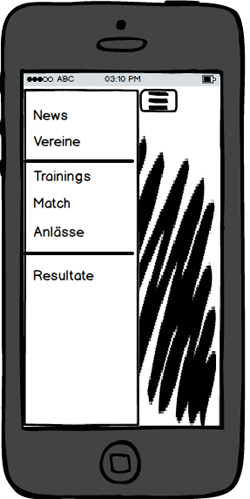
\includegraphics[scale=0.5]{images/mockups/navigation.png}
  \label{fig:mockup_navigation}
}
\subfigure[Einstellungen]{
  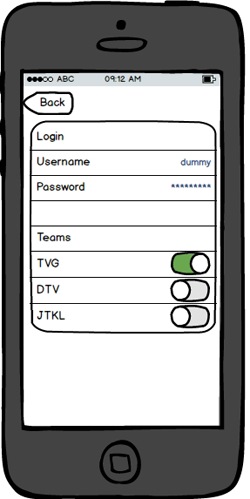
\includegraphics[scale=0.5]{images/mockups/settings.png}
  \label{fig:mockup_settings}
}
\label{fig:mockup_setting}
\caption{Navigation und Einstellungen}
\end{figure}

\newpage
\FloatBarrier
\subsubsection{Berichte}\label{mockup_news}
Als Startseite sollte eine Seite gewählt werden, die etwas Aktuelles anzeigt, somit fiel die Entscheidung auf die Seite mit den Berichten.
\begin{figure}[ht]
\centering
\subfigure[Berichte Übersicht]{
  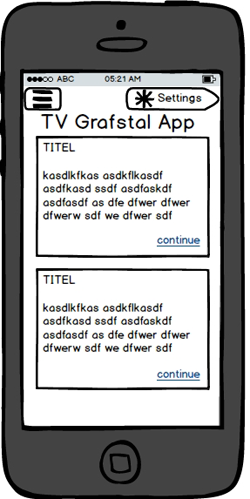
\includegraphics[scale=0.5]{images/mockups/news.png}
  \label{fig:mockup_news_list}
}
\subfigure[Bericht Details]{
  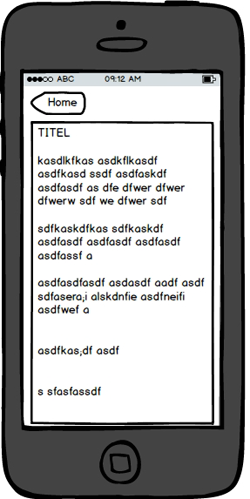
\includegraphics[scale=0.5]{images/mockups/news_detail.png}
  \label{fig:mockup_news_detail}
}
\label{fig:mockup_news}
\caption{Berichte}
\end{figure}

\FloatBarrier
\subsubsection{Vereine}\label{mockup_vereine}
Die Überlegungen zur Gestaltung der Informationen der Vereine sahen so aus:
\begin{figure}[ht]
\centering
\subfigure[Vereine]{
  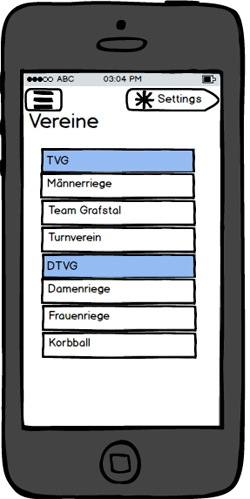
\includegraphics[scale=0.5]{images/mockups/vereine.png}
  \label{fig:mockup_vereine}
}
\subfigure[Verein Details]{
  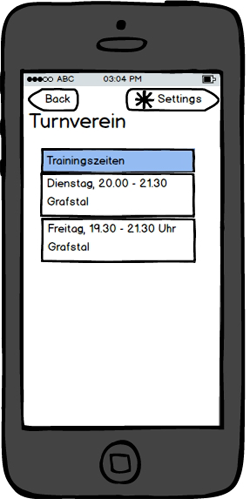
\includegraphics[scale=0.5]{images/mockups/verein_detail.png}
  \label{fig:mockup_verein_detail}
}
\label{fig:mockup_verein}
\caption{Vereine}
\end{figure}

\FloatBarrier
\subsubsection{Veranstaltungen}\label{mockup_singingobjects}
Die verschiedenen Übersichten und Detailsichten der Veranstaltungen sollten ursprünglich so aussehen:
\begin{figure}[ht]
\centering
\subfigure[Anlässe]{
  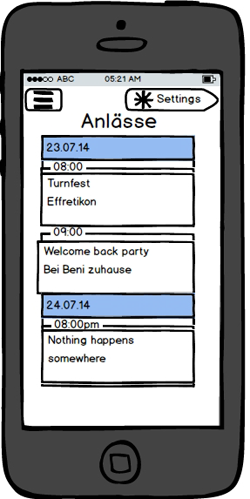
\includegraphics[scale=0.5]{images/mockups/events.png}
  \label{fig:mockup_events}
}
\subfigure[Anlass Details]{
  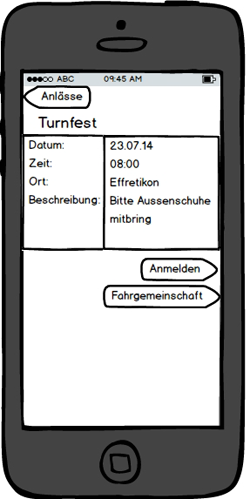
\includegraphics[scale=0.5]{images/mockups/event_detail.png}
  \label{fig:mockup_event_detail}
}
\label{fig:mockup_event}
\caption{Anlässe}
\end{figure}

\begin{figure}[ht]
\centering
\subfigure[Matches]{
  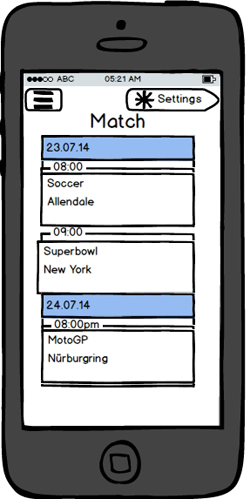
\includegraphics[scale=0.5]{images/mockups/matches.png}
  \label{fig:mockup_matches}
}
\subfigure[Match Details]{
  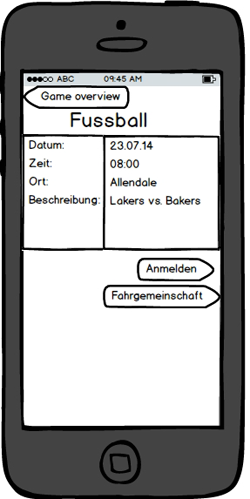
\includegraphics[scale=0.5]{images/mockups/match_detail.png}
  \label{fig:mockup_match_detail}
}
\label{fig:mockup_match}
\caption{Matches}
\end{figure}

\begin{figure}[ht]
\centering
\subfigure[Trainings]{
  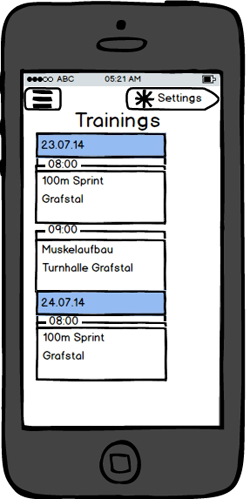
\includegraphics[scale=0.5]{images/mockups/trainings.png}
  \label{fig:mockup_trainings}
}
\subfigure[Training Details]{
  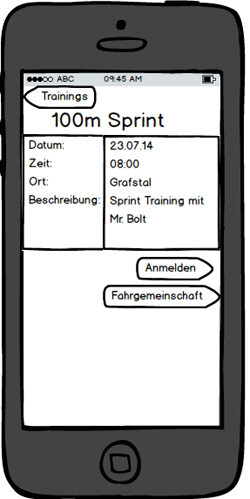
\includegraphics[scale=0.5]{images/mockups/training_detail.png}
  \label{fig:mockup_training_detail}
}
\label{fig:mockup_training}
\caption{Trainings}
\end{figure}

\FloatBarrier
\subsubsection{Resultate}\label{mockup_results}
Das \glossarmark{Mockup} für die Darstellung der Resultate sah eine veranstaltungsspezifische Darstellung vor, wurde dann im späteren Verlauf des Projektes auf eine personenspezifische Übersicht abgeändert. Diese Ansicht war kein Use Case der \glossarmark{Stakeholder} und wurde als möglicher \glossarmark{Begeisterungsfaktor} vom Entwickler hinzugefügt.
\begin{figure}[h]
\centering
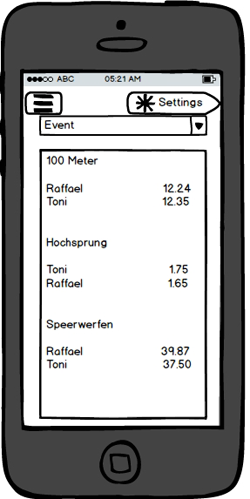
\includegraphics[scale=0.5]{images/mockups/results.png}
\caption{Resultate}
\label{fig:mockup_results}
\end{figure}

\newpage
\FloatBarrier
\subsubsection{Fahrgemeinschaften}\label{mockups_carpools}
Eine der wichtigsten Ansichten, die zu diesem Zeitpunkt nicht auf der Webseite existierte, war jene der Fahrgemeinschaft. An diesem Punkt wurden schon die ersten Überlegungen getroffen, welche Informationen für eine Fahrgemeinschaft relevant sind.
\begin{figure}[ht]
\centering
\subfigure[Fahrgemeinschafen]{
  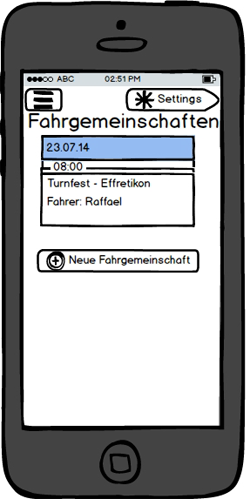
\includegraphics[scale=0.5]{images/mockups/carpools.png}
  \label{fig:mockup_carpools}
}
\subfigure[Fahrgemeinschaft Details]{
  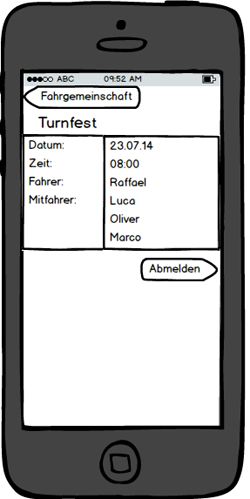
\includegraphics[scale=0.5]{images/mockups/carpool_detail.png}
  \label{fig:mockup_carpool_detail}
}
\label{fig:mockup_carpool}
\caption{Fahrgemeinschaften}
\end{figure}

\begin{figure}[h]
\centering
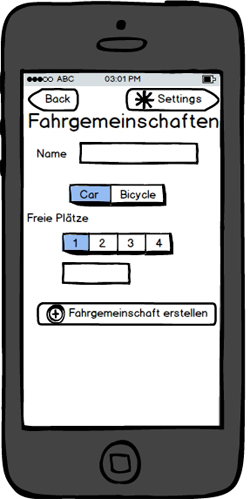
\includegraphics[scale=0.5]{images/mockups/carpool_add.png}
\caption{Fahrgemeinschaft erstellen}
\label{fig:mockup_add_carpool}
\end{figure}

\newpage
\subsection{Anforderungen}\label{anforderungen}
Alle Anforderungen wurden anhand der folgenden Vorlage (siehe Tabelle \ref{table:req_template}) erfasst. Diese Vorlage basiert auf Angaben von \cite{req_eng_book} und wurde mit eigenen Attributen erweitert.

\begin{table}[ht]
\centering
  \begin{tabular}{ l | p{8cm} }
	\hline
	\rowcolor{gray}
	\textbf{ID}			&	Eindeutiger Identifikator\\ \hline
	\textbf{Priorität} 		&	Must, Should, Nice to have\\ \hline
	\textbf{Anforderungstyp}	&	Funktionale Anforderung, Qualitätsanforderung, Randbedingung\\ \hline
	\textbf{Name} 			&	Eindeutiger, charakterisierender Name\\ \hline
	\textbf{Use Case} 		&	Referenz zum zugehörigen Use Case\\ \hline
	\textbf{Beschreibung} 	&	Beschreibung der Anforderung\\ \hline
	\textbf{Begründung} 		&	Bedeutung der Anforderung für das geplante System\\ \hline
	\textbf{Akzeptanz Kriterium}	&	Messbare Abnahmekriterien\\ \hline
	\textbf{Abhängigkeiten} 	&	Referenz zu anderen Anforderungen\\ \hline
	\textbf{Antragssteller} 	&	\glossarmark{Stakeholder}, der um diese Anforderung bittet\\ \hline
	\textbf{Risiken}	 	&	Weisst auf allfällige Risiken betreffend der Anforderungen hin
  \end{tabular}
   \caption{Vorlage für Anforderungen}\label{table:req_template}
\end{table}


Die Beschreibung der Anforderungen wurden zusätzlich mit einer Satzschablone (siehe Abbildung \ref{fig:satzschablone}) aus \cite{req_eng_book} erstellt. Dies hat den Vorteil, dass die Anforderungen normiert und exakt erfasst werden.
\begin{figure}[h]
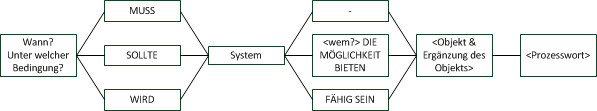
\includegraphics{images/anforderungen/satzschablone.png}
\caption{Satzschablone}
\label{fig:satzschablone}
\end{figure}
\FloatBarrier
Die Abstufungen \emph{muss}, \emph{sollte} und \emph{wird} werden verwendet um die Wichtigkeit der Anforderungen auszudrücken.

\newpage
\FloatBarrier
\subsubsection{Funktionale Anforderungen}\label{func_anforderungen}

\begin{table}[ht]
\centering
  \begin{tabular}{ l | p{8cm} }
	\hline
	\rowcolor{gray}
	\textbf{ID} 			&	\textbf{RE-F1}\\ \hline
	\textbf{Priorität} 		&	Must\\ \hline
	\textbf{Anforderungstyp}	&	Funktionale Anforderung\\ \hline
	\textbf{Name} 			&	Login Möglichkeit bei der Mobile App\\ \hline
	\textbf{Use Case} 		&	-\\ \hline
	\textbf{Beschreibung} 	&	Falls ein Mitglied vom Turnverein auf der Homepage registriert ist, muss das System dem besagten Mitglied die Möglichkeit bieten sich über ein Formular am Backend anzumelden.\\ \hline
	\textbf{Begründung} 		&	Einige Informationen dürfen nur für Mitglieder zugänglich
					gemacht werden. Zusätzlich vereinfacht es das Anmelden, Erstellen
					und Abrufen von benutzerspezifischen Daten\\ \hline
	\textbf{Akzeptanz Kriterium}	&	\begin{enumerate}
					\item Bei bekanntem Username und Passwort muss es dem Mitglied möglich sein, sich beim Backend anzumelden und dann erweiterte	Möglichkeiten und Informationen zu erhalten.
					\item Falls ein unbekannter Username oder das falsche Passwort eingegeben wurden kommt eine entsprechende Fehlermeldung.
					\end{enumerate}
					\\ \hline
	\textbf{Abhängigkeiten} 	&	-\\ \hline
	\textbf{Antragssteller} 	&	Dominic Keller (aktive Mitglieder (U30))\\ \hline
	\textbf{Risiken}	 	&	Falls diese Anforderung nicht erfolgreich implementiert werden kann, gibt es Schwierigkeiten bei sehr vielen anderen Anforderungen.
  \end{tabular}
   \caption{Anforderung RF-F1}\label{table:req_1}
\end{table}

\begin{table}[ht]
\centering
  \begin{tabular}{ l | p{8cm} }
	\hline
	\rowcolor{gray}
	\textbf{ID} 			&	\textbf{RE-F2}\\ \hline
	\textbf{Priorität} 		&	Must\\ \hline
	\textbf{Anforderungstyp}	&	Funktionale Anforderung\\ \hline
	\textbf{Name} 			&	Fahrgemeinschaft erstellen\\ \hline
	\textbf{Use Case} 		&	\nameref{table:use_case_1}\\ \hline
	\textbf{Beschreibung} 	&	Falls das Mitglied angemeldet ist, muss das System dem besagten Mitglied die Möglichkeit bieten über ein Formular eine neue Fahrgemeinschaft zu eröffnen.\\ \hline
	\textbf{Begründung} 		&	Seit einiger Zeit wird vermehrt der Vereins-Chat mit endlosen Diskussionen für Fahrgemeinschaftsorganisationen verwendet, was einige Mitglieder stört und auch nicht der Sinn und Zweck dieses Chats ist. Jedes Mitglied sollte über die App die Möglichkeit haben seine Fahrdienste zur Verfügung zu stellen.\\ \hline
	\textbf{Akzeptanz Kriterium}	&	\begin{enumerate}
					\item Das angemeldete Mitglied kann eine Fahrgemeinschaft eröffnen
					\item Bei ungültigen oder nicht ausreichenden Informationen kommt eine entsprechende Fehlermeldung
					\end{enumerate}
					\\ \hline
	\textbf{Abhängigkeiten} 	&	\nameref{table:req_1}\\ \hline
	\textbf{Antragssteller} 	&	Marco Mathe (Vorstand)\\ \hline
	\textbf{Risiken}	 	&	-
  \end{tabular}
   \caption{Anforderung RF-F2}\label{table:req_2}
\end{table}

\begin{table}[ht]
\centering
  \begin{tabular}{ l | p{8cm} }
	\hline
	\rowcolor{gray}
	\textbf{ID} 			&	\textbf{RE-F3}\\ \hline
	\textbf{Priorität} 		&	Must\\ \hline
	\textbf{Anforderungstyp}	&	Funktionale Anforderung\\ \hline
	\textbf{Name} 			&	Übersicht über Fahrgemeinschaft\\ \hline
	\textbf{Use Case} 		&	\nameref{table:use_case_2}\\ \hline
	\textbf{Beschreibung} 	&	Falls das Mitglied angemeldet ist und eine Fahrgemeinschaft im System besteht, muss das System dem besagten Mitglied die Möglichkeit bieten, eine Liste aller aktuellen Fahrgemeinschaften anzeigen zu lassen.\\ \hline
	\textbf{Begründung} 		&	Das Mitglied benötigt eine Übersicht der aktuellen Fahrgemeinschaften, damit es sich für eine entscheiden kann.\\ \hline
	\textbf{Akzeptanz Kriterium}	&	\begin{enumerate}
					\item Das angemeldete Mitglied kann die Fahrgemeinschaften anzeigen lassen
					\item Das angemeldete Mitglied sieht einen Hinweis, falls es keine Fahrgemeinschaften gibt
					\end{enumerate}
					\\ \hline
	\textbf{Abhängigkeiten} 	&	\nameref{table:req_1}, \nameref{table:req_2}\\ \hline
	\textbf{Antragssteller} 	&	Marco Mathe (Vorstand)\\ \hline
	\textbf{Risiken}	 	&	Falls nur die \nameref{table:req_2} implementiert wird und diese nicht, ist das Fahrgemeinschaft-System nicht funktionsfähig
  \end{tabular}
   \caption{Anforderung RF-F3}\label{table:req_3}
\end{table}

\begin{table}[ht]
\centering
  \begin{tabular}{ l | p{8cm} }
	\hline
	\rowcolor{gray}
	\textbf{ID} 			&	\textbf{RE-F4}\\ \hline
	\textbf{Priorität} 		&	Must\\ \hline
	\textbf{Anforderungstyp}	&	Funktionale Anforderung\\ \hline
	\textbf{Name} 			&	Fahrgemeinschaft beitreten\\ \hline
	\textbf{Use Case} 		&	\nameref{table:use_case_3}\\ \hline
	\textbf{Beschreibung} 	&	Falls das Mitglied angemeldet ist, eine Fahrgemeinschaft im System besteht, das besagte Mitglied noch nicht beigetreten ist und die Fahrgemeinschaft noch Kapazität aufweist, muss das System dem besagten Mitglied die Möglichkeit bieten, sich über einen Knopf bei einer Fahrgemeinschaft einzutragen.\\ \hline
	\textbf{Begründung} 		&	Damit die Fahrgemeinschaften auch funktionieren, muss es den Mitgliedern möglich sein, sich selbständig bei den Fahrgemeinschaften einzutragen.\\ \hline
	\textbf{Akzeptanz Kriterium}	&	\begin{enumerate}
					\item Das angemeldete Mitglied kann einer Fahrgemeinschaft beitreten
					\item Das angemeldete Mitglied kann einer Fahrgemeinschaft nicht erneut beitreten
					\item Das angemeldete Mitglied erhält eine Fehlermeldung falls die Fahrgemeinschaft keine Kapazität mehr aufweist
					\end{enumerate}
					\\ \hline
	\textbf{Abhängigkeiten} 	&	\nameref{table:req_1}, \nameref{table:req_2}, \nameref{table:req_3}\\ \hline
	\textbf{Antragssteller} 	&	Marco Mathe (Vorstand)\\ \hline
	\textbf{Risiken}	 	&	Falls nur die \nameref{table:req_2} und \nameref{table:req_3} implementiert werden und diese nicht, ist das Fahrgemeinschaft-System nicht funktionsfähig
  \end{tabular}
   \caption{Anforderung RF-F4}\label{table:req_4}
\end{table}

\begin{table}[ht]
\centering
  \begin{tabular}{ l | p{8cm} }
	\hline
	\rowcolor{gray}
	\textbf{ID} 			&	\textbf{RE-F5}\\ \hline
	\textbf{Priorität} 		&	Should\\ \hline
	\textbf{Anforderungstyp}	&	Funktionale Anforderung\\ \hline
	\textbf{Name} 			&	Anmelden an Vereinsanlässe\\ \hline
	\textbf{Use Case} 		&	\nameref{table:use_case_4}\\ \hline
	\textbf{Beschreibung} 	&	Falls das Mitglied angemeldet ist, ein Anlass im System besteht und das besagte Mitglied noch nicht angemeldet ist, sollte das System dem besagten Mitglied die Möglichkeit bieten, sich über einen Knopf für den Anlass anzumelden.\\ \hline
	\textbf{Begründung} 		&	Die Anmeldequote der Mitglieder ist nicht so hoch wie erwünscht, durch das Anbieten der Anmelde-Möglichkeit über das App soll das Anmelden vereinfacht und die Anmeldequote erhöht werden.\\ \hline
	\textbf{Akzeptanz Kriterium}	&	\begin{enumerate}
					\item Das angemeldete Mitglied kann sich für einen Anlass anmelden
					\item Das angemeldete Mitglied kann sich für einen Anlass nicht erneut anmelden
					\end{enumerate}
					\\ \hline
	\textbf{Abhängigkeiten} 	&	\nameref{table:req_1}, \nameref{table:req_2}, \nameref{table:req_3}\\ \hline
	\textbf{Antragssteller} 	&	Dominic Keller (aktive Mitglieder (U30))\\ \hline
	\textbf{Risiken}	 	&	-
  \end{tabular}
   \caption{Anforderung RF-F5}\label{table:req_5}
\end{table}

\begin{table}[ht]
\centering
  \begin{tabular}{ l | p{8cm} }
	\hline
	\rowcolor{gray}
	\textbf{ID} 			&	\textbf{RE-F6}\\ \hline
	\textbf{Priorität} 		&	Must\\ \hline
	\textbf{Anforderungstyp}	&	Funktionale Anforderung\\ \hline
	\textbf{Name} 			&	Informationen über Vereinsanlässe\\ \hline
	\textbf{Use Case} 		&	\nameref{table:use_case_5}\\ \hline
	\textbf{Beschreibung} 	&	Falls ein Anlass im System ist, muss das System dem Benutzer der App die Möglichkeit bieten, Informationen über Vereinsanlässe zu erhalten.\\ \hline
	\textbf{Begründung} 		&	Über die App kann man die Informationen schnell und einfach abrufen, somit sollte den Anlässen mehr Beachtung geschenkt werden.\\ \hline
	\textbf{Akzeptanz Kriterium}	&	\begin{enumerate}
					\item Der Benutzer erhält informationen über den ausgewählten Anlass
					\item Der Benutzer sieht einen Hinweis, falls keine Anlässe vorhanden sind
					\end{enumerate}
					\\ \hline
	\textbf{Abhängigkeiten} 	&	-\\ \hline
	\textbf{Antragssteller} 	&	Ivan Sebastiano (Vorstand)\\ \hline
	\textbf{Risiken}	 	&	-
  \end{tabular}
   \caption{Anforderung RF-F6}\label{table:req_6}
\end{table}

\begin{table}[ht]
\centering
  \begin{tabular}{ l | p{8cm} }
	\hline
	\rowcolor{gray}
	\textbf{ID} 			&	\textbf{RE-F7}\\ \hline
	\textbf{Priorität} 		&	Must\\ \hline
	\textbf{Anforderungstyp}	&	Funktionale Anforderung\\ \hline
	\textbf{Name} 			&	Erweiterte Informationen über Vereinsanlässe\\ \hline
	\textbf{Use Case} 		&	\nameref{table:use_case_5}\\ \hline
	\textbf{Beschreibung} 	&	Falls das Mitglied angemeldet ist und ein Anlass im System besteht, sollte das System dem besagten Mitglied die Möglichkeit bieten, zusätzliche Informationen über den Anlass zu erhalten.\\ \hline
	\textbf{Begründung} 		&	Einige Informationen (z. B. Anmelde-Listen) sind aus Datenschutz- oder anderen Gründen nicht für alle Nutzer der App bestimmt und sollten nur angemeldeten Mitgliedern angezeigt werden.\\ \hline
	\textbf{Akzeptanz Kriterium}	&	\begin{enumerate}
					\item Das angemeldete Mitglied sieht die erweiterten Informationen zum Anlass
					\item Nicht angemeldete Mitglieder sehen die erweiterten Informationen zum Anlass nicht
					\end{enumerate}
					\\ \hline
	\textbf{Abhängigkeiten} 	&	\nameref{table:req_1}, \nameref{table:req_6}\\ \hline
	\textbf{Antragssteller} 	&	Ivan Sebastiano (Vorstand)\\ \hline
	\textbf{Risiken}	 	&	-
  \end{tabular}
   \caption{Anforderung RF-F7}\label{table:req_7}
\end{table}

\begin{table}[ht]
\centering
  \begin{tabular}{ l | p{8cm} }
	\hline
	\rowcolor{gray}
	\textbf{ID} 			&	\textbf{RE-F8}\\ \hline
	\textbf{Priorität} 		&	Must\\ \hline
	\textbf{Anforderungstyp}	&	Funktionale Anforderung\\ \hline
	\textbf{Name} 			&	Informationen über Vereine und Riegen\\ \hline
	\textbf{Use Case} 		&	\nameref{table:use_case_6}\\ \hline
	\textbf{Beschreibung} 	&	Das System muss dem Benutzer der App die Möglichkeit bieten, Informationen über die verschiedenen Vereine und Riegen zu erhalten.\\ \hline
	\textbf{Begründung} 		&	Die App ist nicht nur für die Mitglieder des Vereins sondern auch für Aussenstehende und sollte auch zu Werbezwecken dienen. Jeder kann aktuelle Trainingszeiten und Inhalte der Trainings anschauen und erhält Kontaktinformationen.\\ \hline
	\textbf{Akzeptanz Kriterium}	&	\begin{enumerate}
					\item Der Benutzer erhält Informationen über die verschiedenen Vereine und Riegen
					\end{enumerate}
					\\ \hline
	\textbf{Abhängigkeiten} 	&	-\\ \hline
	\textbf{Antragssteller} 	&	Ivan Sebastiano (Vorstand)\\ \hline
	\textbf{Risiken}	 	&	-
  \end{tabular}
   \caption{Anforderung RF-F8}\label{table:req_8}
\end{table}

\begin{table}[ht]
\centering
  \begin{tabular}{ l | p{8cm} }
	\hline
	\rowcolor{gray}
	\textbf{ID} 			&	\textbf{RE-F9}\\ \hline
	\textbf{Priorität} 		&	Must\\ \hline
	\textbf{Anforderungstyp}	&	Funktionale Anforderung\\ \hline
	\textbf{Name} 			&	Aktuellen Berichte\\ \hline
	\textbf{Use Case} 		&	\nameref{table:use_case_6}\\ \hline
	\textbf{Beschreibung} 	&	Das System muss dem Benutzer der App die Möglichkeit bieten, aktuellen Berichte von den einzelnen Anlässen oder Vereinen lesen zu können.\\ \hline
	\textbf{Begründung} 		&	Die App ist nicht nur für die Mitglieder des Vereins sondern auch für Aussenstehende und sollte auch zu Werbezwecken dienen. In den Berichten wird über aktuelle Anlässe und Geschehnisse geschrieben, ganz nach dem Motto 'Tue gutes und sprich darüber'.\\ \hline
	\textbf{Akzeptanz Kriterium}	&	\begin{enumerate}
					\item Der Benutzer kann die aktuellen Berichte lesen
					\end{enumerate}
					\\ \hline
	\textbf{Abhängigkeiten} 	&	-\\ \hline
	\textbf{Antragssteller} 	&	Dominic Keller (aktive Mitglieder (U30))\\ \hline
	\textbf{Risiken}	 	&	-
  \end{tabular}
   \caption{Anforderung RF-F9}\label{table:req_9}
\end{table}

\begin{table}[ht]
\centering
  \begin{tabular}{ l | p{8cm} }
	\hline
	\rowcolor{gray}
	\textbf{ID} 			&	\textbf{RE-F10}\\ \hline
	\textbf{Priorität} 		&	Nice to have\\ \hline
	\textbf{Anforderungstyp}	&	Funktionale Anforderung\\ \hline
	\textbf{Name} 			&	Push-Nachrichten versenden\\ \hline
	\textbf{Use Case} 		&	-\\ \hline
	\textbf{Beschreibung} 	&	Falls das Mitglied angemeldet ist, Push-Nachrichten zugelassen werden und eine solche vom Backend versendet wurde, sollte das System dem besagten Mitglied eine Push Notification zustellen.\\ \hline
	\textbf{Begründung} 		&	Trainingsverantwortliche und Vorstandsmitglieder können die Mitglieder mit Push-Nachrichten schneller über kurzfristige Änderungen informieren.\\ \hline
	\textbf{Akzeptanz Kriterium}	&	\begin{enumerate}
					\item Das angemeldete Mitglied erhält die Push-Nachrichten
					\end{enumerate}
					\\ \hline
	\textbf{Abhängigkeiten} 	&	\nameref{table:req_1}\\ \hline
	\textbf{Antragssteller} 	&	Oliver Zimmermann (Trainingsverantwortliche)\\ \hline
	\textbf{Risiken}	 	&	-
  \end{tabular}
   \caption{Anforderung RF-F10}\label{table:req_10}
\end{table}

\newpage
\FloatBarrier
\subsubsection{Qualitätsanforderung}\label{non_func_anforderungen}

\begin{table}[ht]
\centering
  \begin{tabular}{ l | p{8cm} }
	\hline
	\rowcolor{gray}
	\textbf{ID} 			&	\textbf{RE-NF1}\\ \hline
	\textbf{Priorität} 		&	Must\\ \hline
	\textbf{Anforderungstyp}	&	Qualitätsanforderung\\ \hline
	\textbf{Name} 			&	Unterstützung von Android\\ \hline
	\textbf{Use Case} 		&	-\\ \hline
	\textbf{Beschreibung} 	&	Das System muss fähig sein, auf Android Geräten zu laufen.\\ \hline
	\textbf{Begründung} 		&	Die Statistik der aktuellen Homepage zeigt, dass über 50\% der Zugriffe über Mobiltelefone und Tablet von Android Plattformen stammen.\\ \hline
	\textbf{Akzeptanz Kriterium}	&	\begin{enumerate}
					\item Ein Nutzer mit einem Android Mobiltelefon kann die App öffnen und verwenden
					\end{enumerate}
					\\ \hline
	\textbf{Abhängigkeiten} 	&	-\\ \hline
	\textbf{Antragssteller} 	&	Dominic Keller (aktive Mitglieder (U30))\\ \hline
	\textbf{Risiken}	 	&	-
  \end{tabular}
   \caption{Qualitätsanforderung RF-NF1}\label{table:req_nf_1}
\end{table}

\begin{table}[ht]
\centering
  \begin{tabular}{ l | p{8cm} }
	\hline
	\rowcolor{gray}
	\textbf{ID} 			&	\textbf{RE-NF2}\\ \hline
	\textbf{Priorität} 		&	Must\\ \hline
	\textbf{Anforderungstyp}	&	Qualitätsanforderung\\ \hline
	\textbf{Name} 			&	Unterstützung von iOS\\ \hline
	\textbf{Use Case} 		&	-\\ \hline
	\textbf{Beschreibung} 	&	Das System muss fähig sein, auf iOS Geräten zu laufen.\\ \hline
	\textbf{Begründung} 		&	Die Statistik der aktuellen Homepage zeigt, dass gut 43\% der Zugriffe über Mobiltelefone und Tablet von iOS Plattformen stammen.\\ \hline
	\textbf{Akzeptanz Kriterium}	&	\begin{enumerate}
					\item Ein Nutzer mit einem iPhone kann die App öffnen und verwenden
					\end{enumerate}
					\\ \hline
	\textbf{Abhängigkeiten} 	&	-\\ \hline
	\textbf{Antragssteller} 	&	Marco Mathe (Vorstand)\\ \hline
	\textbf{Risiken}	 	&	-
  \end{tabular}
   \caption{Qualitätsanforderung RF-NF2}\label{table:req_nf_2}
\end{table}


